\PassOptionsToPackage{unicode=true}{hyperref} % options for packages loaded elsewhere
\PassOptionsToPackage{hyphens}{url}
%
\documentclass[english,man]{apa6}
\usepackage{lmodern}
\usepackage{amssymb,amsmath}
\usepackage{ifxetex,ifluatex}
\usepackage{fixltx2e} % provides \textsubscript
\ifnum 0\ifxetex 1\fi\ifluatex 1\fi=0 % if pdftex
  \usepackage[T1]{fontenc}
  \usepackage[utf8]{inputenc}
  \usepackage{textcomp} % provides euro and other symbols
\else % if luatex or xelatex
  \usepackage{unicode-math}
  \defaultfontfeatures{Ligatures=TeX,Scale=MatchLowercase}
\fi
% use upquote if available, for straight quotes in verbatim environments
\IfFileExists{upquote.sty}{\usepackage{upquote}}{}
% use microtype if available
\IfFileExists{microtype.sty}{%
\usepackage[]{microtype}
\UseMicrotypeSet[protrusion]{basicmath} % disable protrusion for tt fonts
}{}
\IfFileExists{parskip.sty}{%
\usepackage{parskip}
}{% else
\setlength{\parindent}{0pt}
\setlength{\parskip}{6pt plus 2pt minus 1pt}
}
\usepackage{hyperref}
\hypersetup{
            pdftitle={Tool Demo: An R package for detecting biases in word embeddings},
            pdfauthor={Chung-hong Chan1},
            pdfkeywords={word embedding, bias, fairness, gender stereotypes},
            pdfborder={0 0 0},
            breaklinks=true}
\urlstyle{same}  % don't use monospace font for urls
\usepackage{color}
\usepackage{fancyvrb}
\newcommand{\VerbBar}{|}
\newcommand{\VERB}{\Verb[commandchars=\\\{\}]}
\DefineVerbatimEnvironment{Highlighting}{Verbatim}{commandchars=\\\{\}}
% Add ',fontsize=\small' for more characters per line
\usepackage{framed}
\definecolor{shadecolor}{RGB}{248,248,248}
\newenvironment{Shaded}{\begin{snugshade}}{\end{snugshade}}
\newcommand{\AlertTok}[1]{\textcolor[rgb]{0.94,0.16,0.16}{#1}}
\newcommand{\AnnotationTok}[1]{\textcolor[rgb]{0.56,0.35,0.01}{\textbf{\textit{#1}}}}
\newcommand{\AttributeTok}[1]{\textcolor[rgb]{0.77,0.63,0.00}{#1}}
\newcommand{\BaseNTok}[1]{\textcolor[rgb]{0.00,0.00,0.81}{#1}}
\newcommand{\BuiltInTok}[1]{#1}
\newcommand{\CharTok}[1]{\textcolor[rgb]{0.31,0.60,0.02}{#1}}
\newcommand{\CommentTok}[1]{\textcolor[rgb]{0.56,0.35,0.01}{\textit{#1}}}
\newcommand{\CommentVarTok}[1]{\textcolor[rgb]{0.56,0.35,0.01}{\textbf{\textit{#1}}}}
\newcommand{\ConstantTok}[1]{\textcolor[rgb]{0.00,0.00,0.00}{#1}}
\newcommand{\ControlFlowTok}[1]{\textcolor[rgb]{0.13,0.29,0.53}{\textbf{#1}}}
\newcommand{\DataTypeTok}[1]{\textcolor[rgb]{0.13,0.29,0.53}{#1}}
\newcommand{\DecValTok}[1]{\textcolor[rgb]{0.00,0.00,0.81}{#1}}
\newcommand{\DocumentationTok}[1]{\textcolor[rgb]{0.56,0.35,0.01}{\textbf{\textit{#1}}}}
\newcommand{\ErrorTok}[1]{\textcolor[rgb]{0.64,0.00,0.00}{\textbf{#1}}}
\newcommand{\ExtensionTok}[1]{#1}
\newcommand{\FloatTok}[1]{\textcolor[rgb]{0.00,0.00,0.81}{#1}}
\newcommand{\FunctionTok}[1]{\textcolor[rgb]{0.00,0.00,0.00}{#1}}
\newcommand{\ImportTok}[1]{#1}
\newcommand{\InformationTok}[1]{\textcolor[rgb]{0.56,0.35,0.01}{\textbf{\textit{#1}}}}
\newcommand{\KeywordTok}[1]{\textcolor[rgb]{0.13,0.29,0.53}{\textbf{#1}}}
\newcommand{\NormalTok}[1]{#1}
\newcommand{\OperatorTok}[1]{\textcolor[rgb]{0.81,0.36,0.00}{\textbf{#1}}}
\newcommand{\OtherTok}[1]{\textcolor[rgb]{0.56,0.35,0.01}{#1}}
\newcommand{\PreprocessorTok}[1]{\textcolor[rgb]{0.56,0.35,0.01}{\textit{#1}}}
\newcommand{\RegionMarkerTok}[1]{#1}
\newcommand{\SpecialCharTok}[1]{\textcolor[rgb]{0.00,0.00,0.00}{#1}}
\newcommand{\SpecialStringTok}[1]{\textcolor[rgb]{0.31,0.60,0.02}{#1}}
\newcommand{\StringTok}[1]{\textcolor[rgb]{0.31,0.60,0.02}{#1}}
\newcommand{\VariableTok}[1]{\textcolor[rgb]{0.00,0.00,0.00}{#1}}
\newcommand{\VerbatimStringTok}[1]{\textcolor[rgb]{0.31,0.60,0.02}{#1}}
\newcommand{\WarningTok}[1]{\textcolor[rgb]{0.56,0.35,0.01}{\textbf{\textit{#1}}}}
\usepackage{longtable,booktabs}
% Fix footnotes in tables (requires footnote package)
\IfFileExists{footnote.sty}{\usepackage{footnote}\makesavenoteenv{longtable}}{}
\usepackage{graphicx,grffile}
\makeatletter
\def\maxwidth{\ifdim\Gin@nat@width>\linewidth\linewidth\else\Gin@nat@width\fi}
\def\maxheight{\ifdim\Gin@nat@height>\textheight\textheight\else\Gin@nat@height\fi}
\makeatother
% Scale images if necessary, so that they will not overflow the page
% margins by default, and it is still possible to overwrite the defaults
% using explicit options in \includegraphics[width, height, ...]{}
\setkeys{Gin}{width=\maxwidth,height=\maxheight,keepaspectratio}
\setlength{\emergencystretch}{3em}  % prevent overfull lines
\providecommand{\tightlist}{%
  \setlength{\itemsep}{0pt}\setlength{\parskip}{0pt}}
\setcounter{secnumdepth}{0}

% set default figure placement to htbp
\makeatletter
\def\fps@figure{htbp}
\makeatother

% Manuscript styling
\usepackage{upgreek}
\captionsetup{font=singlespacing,justification=justified}

% Table formatting
\usepackage{longtable}
\usepackage{lscape}
% \usepackage[counterclockwise]{rotating}   % Landscape page setup for large tables
\usepackage{multirow}		% Table styling
\usepackage{tabularx}		% Control Column width
\usepackage[flushleft]{threeparttable}	% Allows for three part tables with a specified notes section
\usepackage{threeparttablex}            % Lets threeparttable work with longtable

% Create new environments so endfloat can handle them
% \newenvironment{ltable}
%   {\begin{landscape}\begin{center}\begin{threeparttable}}
%   {\end{threeparttable}\end{center}\end{landscape}}
\newenvironment{lltable}{\begin{landscape}\begin{center}\begin{ThreePartTable}}{\end{ThreePartTable}\end{center}\end{landscape}}

% Enables adjusting longtable caption width to table width
% Solution found at http://golatex.de/longtable-mit-caption-so-breit-wie-die-tabelle-t15767.html
\makeatletter
\newcommand\LastLTentrywidth{1em}
\newlength\longtablewidth
\setlength{\longtablewidth}{1in}
\newcommand{\getlongtablewidth}{\begingroup \ifcsname LT@\roman{LT@tables}\endcsname \global\longtablewidth=0pt \renewcommand{\LT@entry}[2]{\global\advance\longtablewidth by ##2\relax\gdef\LastLTentrywidth{##2}}\@nameuse{LT@\roman{LT@tables}} \fi \endgroup}

% \setlength{\parindent}{0.5in}
% \setlength{\parskip}{0pt plus 0pt minus 0pt}

% \usepackage{etoolbox}
\makeatletter
\patchcmd{\HyOrg@maketitle}
  {\section{\normalfont\normalsize\abstractname}}
  {\section*{\normalfont\normalsize\abstractname}}
  {}{\typeout{Failed to patch abstract.}}
\patchcmd{\HyOrg@maketitle}
  {\section{\protect\normalfont{\@title}}}
  {\section*{\protect\normalfont{\@title}}}
  {}{\typeout{Failed to patch title.}}
\makeatother
\shorttitle{DETECTING BIASES IN WORD EMBEDDINGS}
\keywords{word embedding, bias, fairness, gender stereotypes}
\DeclareDelayedFloatFlavor{ThreePartTable}{table}
\DeclareDelayedFloatFlavor{lltable}{table}
\DeclareDelayedFloatFlavor*{longtable}{table}
\makeatletter
\renewcommand{\efloat@iwrite}[1]{\immediate\expandafter\protected@write\csname efloat@post#1\endcsname{}}
\makeatother
\usepackage{lineno}

\linenumbers
\usepackage{csquotes}
\ifnum 0\ifxetex 1\fi\ifluatex 1\fi=0 % if pdftex
  \usepackage[shorthands=off,main=english]{babel}
\else
  % load polyglossia as late as possible as it *could* call bidi if RTL lang (e.g. Hebrew or Arabic)
  \usepackage{polyglossia}
  \setmainlanguage[]{english}
\fi

\title{Tool Demo: An R package for detecting biases in word embeddings}
\author{Chung-hong Chan\textsuperscript{1}}
\date{}


\authornote{

The development of this package was partly supported by a research grant from the Federal Ministry for Family Affairs, Senior Citizens, Women and Youth (Bundesministerium für Familie, Senioren, Frauen und Jugend), the Federal Republic of Germany.

Correspondence concerning this article should be addressed to Chung-hong Chan, A5, 6 (section A), 68159 Mannheim, Germany. E-mail: \href{mailto:chung-hong.chan@mzes.uni-mannheim.de}{\nolinkurl{chung-hong.chan@mzes.uni-mannheim.de}}

}

\affiliation{\vspace{0.5cm}\textsuperscript{1} Mannheimer Zentrum für Europäische Sozialforschung}

\abstract{
This paper shows how the R package sweater can be used to detect biases in word embeddings. The package provides highly optimized functions to calculate the following bias metrics: mean average cosine similarity, relative norm distance, SemAxis, normalized association score, relative negative sentiment bias, embedding coherence test and word embedding association test. Using two public available word embeddings trained on media content, this paper demonstrates how sweater can be used to study implicit gender stereotypes.
}



\begin{document}
\maketitle

\hypertarget{statement-of-need}{%
\section{Statement of need}\label{statement-of-need}}

The goal of the R package \texttt{sweater} is to detect (implicit) biases in word embeddings. The importance of detecting biases in word embeddings is twofold. First, pretrained, biased word embeddings deployed in real-life machine learning systems can pose fairness concerns (Boyarskaya, Olteanu, \& Crawford, 2020; Packer, Mitchell, Guajardo-Céspedes, \& Halpern, 2018). Second, biases in word embeddings reflect the biases in the original training material. Social scientists, communication researchers included, have exploited these methods to quantify (implicit) media biases by extracting biases from word embeddings locally trained on large text corpora (e.g.~Kroon, Trilling, \& Raats, 2020; Knoche, Popović, Lemmerich, \& Strohmaier, 2019; Sales, Balby, \& Veloso, 2019). Biases in word embedding can be understood through the implicit social cognition model of media priming (Arendt, 2013). In this model, implicit stereotypes are defined as the \enquote{strength of the automatic association between a group concept (e.g., minority group) and an attribute (e.g., criminal).} (Arendt, 2013, p. 832) All of these bias detection methods are based on the strength of association between a concept (or a target) and an attribute in embedding spaces.

Previously, the software of these methods is only scatteredly available as the addendum of the original papers and was implemented in different languages (Java, Python, etc.). \texttt{sweater} provides several of these bias detection methods in one unified package with a consistent R interface (R Core Team, 2021). Also, some provided methods in \texttt{sweater} are implemented in C++ and interfaced to R using the Rcpp package (Eddelbuettel, 2013). These heavily optimized methods, such as the Word Embedding Association Test (WEAT) (Caliskan, Bryson, \& Narayanan, 2017), are significantly faster than the same methods implemented in interpreted languages.

In the usage section below, we demonstrated how the package can be used to detect biases and reproduce some published findings.

\hypertarget{usage}{%
\section{Usage}\label{usage}}

\hypertarget{word-embeddings}{%
\subsection{Word Embeddings}\label{word-embeddings}}

The input word embedding \(w\) is a dense \(m\times n\) matrix, where \(m\) is the total size of the vocabulary in the training corpus and \(n\) is the vector dimension size. Let \(v_x\) denote a row vector of \(w\), the word vector of the word \(x\).

\texttt{sweater} supports two types of \(w\). For locally trained word embeddings, word embedding outputs from the R packages \emph{word2vec} (Wijffels, 2021), \emph{rsparse} (Selivanov, 2020) and \emph{text2vec} (Selivanov et al., 2020) are directly supported.\footnote{The vignette of \emph{text2vec} provides a guide on how to locally train word embeddings using the GLoVE algorithm (Pennington, Socher, \& Manning, 2014) on a large corpus from R. \url{https://cran.r-project.org/web/packages/text2vec/vignettes/glove.html}} For pretrained word embeddings obtained online,\footnote{For example, the pretrained GLoVE word embeddings provided in \url{https://nlp.stanford.edu/projects/glove/}, pretrained word2vec word embeddings provided in \url{https://wikipedia2vec.github.io/wikipedia2vec/pretrained/} and fastText word embeddings provided in \url{https://fasttext.cc/docs/en/english-vectors.html}.} they are usually provided in the so-called \enquote{word2vec} file format and \texttt{sweater}'s function \texttt{read\_word2vec} reads those files into the supported matrix format.

\hypertarget{query}{%
\subsection{Query}\label{query}}

\texttt{sweater} uses the concept of \emph{query} (Badilla, Bravo-Marquez, \& Pérez, 2020) to study the biases in \(w\). A query contains two or more sets of seed words with at least one set of \emph{target words} and one set of \emph{attribute words}. \texttt{sweater} uses the \(\mathcal{S}\mathcal{T}\mathcal{A}\mathcal{B}\) notation from Brunet, Alkalay-Houlihan, Anderson, and Zemel (2019) to form a query.

Target words are words that \textbf{should} have no bias. They are denoted as wordsets \(\mathcal{S}\) and \(\mathcal{T}\). All methods require \(\mathcal{S}\) while \(\mathcal{T}\) is only required for WEAT. For instance, the study of gender stereotypes in academic pursuits by Caliskan et al. (2017) used \(\mathcal{S} = \{math, algebra, geometry, calculus, equations, computation, numbers, addition\}\) and \(\mathcal{T}= \{poetry, art, dance, literature, novel, symphony, drama, sculpture\}\).

Attribute words are words that have known properties in relation to the bias. They are denoted as wordsets \(\mathcal{A}\) and \(\mathcal{B}\). All methods require both wordsets except Mean Average Cosine Similarity (Manzini, Lim, Tsvetkov, \& Black, 2019). For instance, the study of gender stereotypes by Caliskan et al. (2017) used \(\mathcal{A} = \{he, son, his, him, father, man, boy, himself, male, ...\}\) and \(\mathcal{B} = \{she, daughter, hers, her, mother, woman, girl, herself, female, ...\}\). In some applications, popular off-the-shelf sentiment dictionaries can also be used as \(\mathcal{A}\) and \(\mathcal{B}\) (e.g.~Sweeney \& Najafian, 2020). That being said, it is up to the researchers to select and derive these seed words in a query. However, the selection of seed words has been shown to be the most consequential part of the entire analysis (Antoniak \& Mimno, 2021; Du, Fang, \& Nguyen, 2021). Please read Antoniak and Mimno (2021) for recommendations.

\hypertarget{supported-methods}{%
\subsection{Supported methods}\label{supported-methods}}

Table \ref{tab:t1} lists all methods supported by \texttt{sweater}. As Relative Norm Distance, SemAxis, Normalized Association Score, and Embedding Coherence Test are all distance-based measures, only Relative Norm Distance is demonstrated below.

\begin{longtable}[]{@{}llll@{}}
\caption{\label{tab:t1} All methods supported by \texttt{sweater}}\tabularnewline
\toprule
\begin{minipage}[b]{0.39\columnwidth}\raggedright
Method\strut
\end{minipage} & \begin{minipage}[b]{0.21\columnwidth}\raggedright
Target words\strut
\end{minipage} & \begin{minipage}[b]{0.21\columnwidth}\raggedright
Attribute words\strut
\end{minipage} & \begin{minipage}[b]{0.08\columnwidth}\raggedright
shorthand\strut
\end{minipage}\tabularnewline
\midrule
\endfirsthead
\toprule
\begin{minipage}[b]{0.39\columnwidth}\raggedright
Method\strut
\end{minipage} & \begin{minipage}[b]{0.21\columnwidth}\raggedright
Target words\strut
\end{minipage} & \begin{minipage}[b]{0.21\columnwidth}\raggedright
Attribute words\strut
\end{minipage} & \begin{minipage}[b]{0.08\columnwidth}\raggedright
shorthand\strut
\end{minipage}\tabularnewline
\midrule
\endhead
\begin{minipage}[t]{0.39\columnwidth}\raggedright
Mean Average Cosine Similarity (Manzini et al., 2019)\strut
\end{minipage} & \begin{minipage}[t]{0.21\columnwidth}\raggedright
\(\mathcal{S}\)\strut
\end{minipage} & \begin{minipage}[t]{0.21\columnwidth}\raggedright
\(\mathcal{A}\)\strut
\end{minipage} & \begin{minipage}[t]{0.08\columnwidth}\raggedright
\texttt{mac}\strut
\end{minipage}\tabularnewline
\begin{minipage}[t]{0.39\columnwidth}\raggedright
Relative Norm Distance (Garg, Schiebinger, Jurafsky, \& Zou, 2018)\strut
\end{minipage} & \begin{minipage}[t]{0.21\columnwidth}\raggedright
\(\mathcal{S}\)\strut
\end{minipage} & \begin{minipage}[t]{0.21\columnwidth}\raggedright
\(\mathcal{A}\), \(\mathcal{B}\)\strut
\end{minipage} & \begin{minipage}[t]{0.08\columnwidth}\raggedright
\texttt{rnd}\strut
\end{minipage}\tabularnewline
\begin{minipage}[t]{0.39\columnwidth}\raggedright
SemAxis (An, Kwak, \& Ahn, 2018)\strut
\end{minipage} & \begin{minipage}[t]{0.21\columnwidth}\raggedright
\(\mathcal{S}\)\strut
\end{minipage} & \begin{minipage}[t]{0.21\columnwidth}\raggedright
\(\mathcal{A}\), \(\mathcal{B}\)\strut
\end{minipage} & \begin{minipage}[t]{0.08\columnwidth}\raggedright
\texttt{semaxis}\strut
\end{minipage}\tabularnewline
\begin{minipage}[t]{0.39\columnwidth}\raggedright
Normalized Association Score (Caliskan et al., 2017)\strut
\end{minipage} & \begin{minipage}[t]{0.21\columnwidth}\raggedright
\(\mathcal{S}\)\strut
\end{minipage} & \begin{minipage}[t]{0.21\columnwidth}\raggedright
\(\mathcal{A}\), \(\mathcal{B}\)\strut
\end{minipage} & \begin{minipage}[t]{0.08\columnwidth}\raggedright
\texttt{nas}\strut
\end{minipage}\tabularnewline
\begin{minipage}[t]{0.39\columnwidth}\raggedright
Embedding Coherence Test (Dev \& Phillips, 2019)\strut
\end{minipage} & \begin{minipage}[t]{0.21\columnwidth}\raggedright
\(\mathcal{S}\)\strut
\end{minipage} & \begin{minipage}[t]{0.21\columnwidth}\raggedright
\(\mathcal{A}\), \(\mathcal{B}\)\strut
\end{minipage} & \begin{minipage}[t]{0.08\columnwidth}\raggedright
\texttt{ect}\strut
\end{minipage}\tabularnewline
\begin{minipage}[t]{0.39\columnwidth}\raggedright
Relative Negative Sentiment Bias (Sweeney \& Najafian, 2020)\strut
\end{minipage} & \begin{minipage}[t]{0.21\columnwidth}\raggedright
\(\mathcal{S}\)\strut
\end{minipage} & \begin{minipage}[t]{0.21\columnwidth}\raggedright
\(\mathcal{A}\), \(\mathcal{B}\)\strut
\end{minipage} & \begin{minipage}[t]{0.08\columnwidth}\raggedright
\texttt{rnsb}\strut
\end{minipage}\tabularnewline
\begin{minipage}[t]{0.39\columnwidth}\raggedright
Word Embedding Association Test (Caliskan et al., 2017)\strut
\end{minipage} & \begin{minipage}[t]{0.21\columnwidth}\raggedright
\(\mathcal{S}\), \(\mathcal{T}\)\strut
\end{minipage} & \begin{minipage}[t]{0.21\columnwidth}\raggedright
\(\mathcal{A}\), \(\mathcal{B}\)\strut
\end{minipage} & \begin{minipage}[t]{0.08\columnwidth}\raggedright
\texttt{weat}\strut
\end{minipage}\tabularnewline
\bottomrule
\end{longtable}

\hypertarget{examples}{%
\section{Examples}\label{examples}}

In the following examples, the publicly available word2vec word embeddings trained on the Google News corpus is used (Mikolov, Sutskever, Chen, Corrado, \& Dean, 2013). \texttt{sweater} provides a unified interface for making query, calculating effect size, and plotting result. Three functions are used:

\begin{itemize}
\tightlist
\item
  \texttt{query} for making query. It follows a template of \texttt{method(w,\ S\_words,\ T\_words,\ A\_words,\ B\_words,\ method)} for a query.
\item
  \texttt{calculate\_es} for calcuting effect size which represents the overall bias of \(w\) based on the query
\item
  \texttt{plot} for visualizing the result of a query
\end{itemize}

The argument \texttt{method} of the function \texttt{query} determines which method to use (see Table \ref{tab:t1} for the list of shorthands). By default, it is set to \enquote{guess}, i.e.~the function select the appropriate method for you based on your provided \(\mathcal{S}\), \(\mathcal{T}\), \(\mathcal{A}\), and \(\mathcal{B}\).

\hypertarget{mean-average-cosine-similarity}{%
\subsection{Mean Average Cosine Similarity}\label{mean-average-cosine-similarity}}

Average cosine similarity (Manzini et al., 2019) is calculated as the mean cosine similarity between the word vector of a target word \(v_s\) where \(s \in \mathcal{S}\) and that of all terms in the attribute wordset \({\mathcal{A}}\). The same method was deployed in Kroon et al. (2020).

The average cosine similarity of many occupation words in \(\mathcal{S}\) are calculated against a wordset \(\mathcal{A}\) of attribute words related to male.

The code below shows how to conduct a query using the \texttt{query} function. When only \(\mathcal{S}\) and \(\mathcal{A}\) are provided, the function assumes that the query calls for calcuting average cosine similarity. The function returns an S3 object.

In an interactive session, printing the S3 object shows the effect size and other functions (or more accurately, S3 methods) that can further process the object (Figure \ref{fig:interactive}).

\begin{figure}
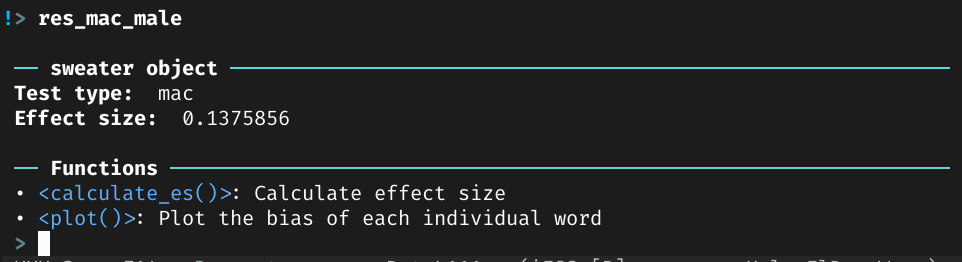
\includegraphics[width=3.21in]{sweaterf1} \caption{The printed S3 object produced with `query` in an R interactive session}\label{fig:interactive}
\end{figure}

For most of the functions, the returned S3 object contains a slot \texttt{P}, which stores the bias of each word (e.g.~\texttt{res\_mac\_male\$P}). The average cosine similarity values are \texttt{P} in this case. The function \texttt{plot} can be used to visualize \texttt{P} as a Cleveland Dot Plot (Figure \ref{fig:acs}).

\begin{Shaded}
\begin{Highlighting}[]
\KeywordTok{plot}\NormalTok{(res_mac_male)}
\end{Highlighting}
\end{Shaded}

\begin{figure}
\centering
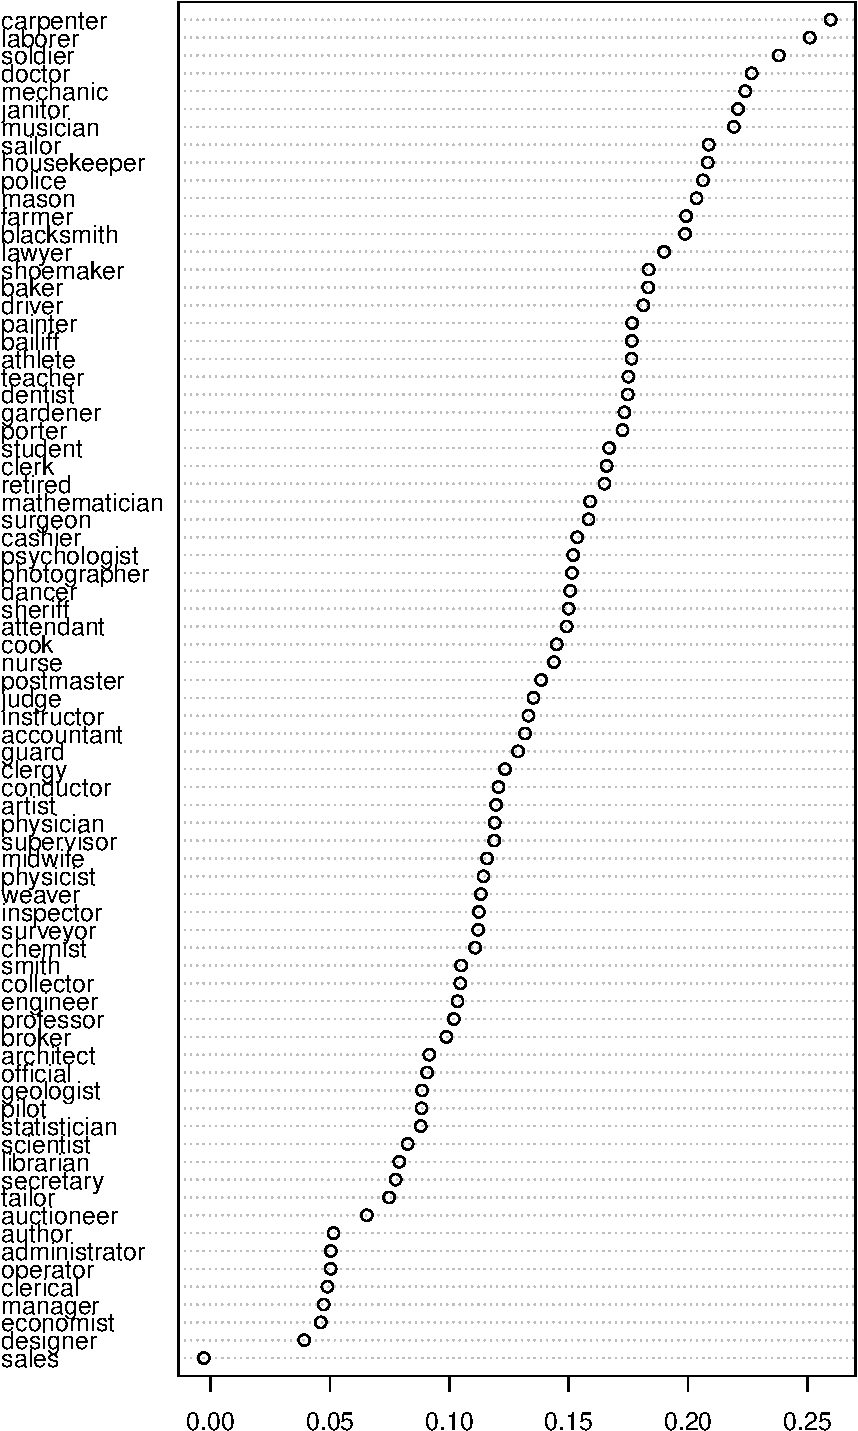
\includegraphics{ica_files/figure-latex/acs-1.pdf}
\caption{\label{fig:acs}Bias of words in the target wordset according to average cosine similarity}
\end{figure}

The effect size, mean average cosine similarity, is the mean value of all average cosine similarity values.

\begin{Shaded}
\begin{Highlighting}[]
\KeywordTok{calculate_es}\NormalTok{(res_mac_male)}
\end{Highlighting}
\end{Shaded}

\begin{verbatim}
## [1] 0.1375856
\end{verbatim}

\hypertarget{relative-norm-distance}{%
\subsection{Relative Norm Distance}\label{relative-norm-distance}}

Relative norm distance (RND) (Garg et al., 2018) is calculated with two sets of attribute words. The following analysis reproduces the calculation of \enquote{women bias} values in Garg et al. (2018). Compared with average cosine similarity, RND appears to be reflecting the underlying gender bias more accurately (Figure \ref{fig:rnd}).

\begin{Shaded}
\begin{Highlighting}[]
\NormalTok{B <-}\StringTok{ }\KeywordTok{c}\NormalTok{(}\StringTok{"she"}\NormalTok{, }\StringTok{"daughter"}\NormalTok{, }\StringTok{"hers"}\NormalTok{, }\StringTok{"her"}\NormalTok{, }\StringTok{"mother"}\NormalTok{, }\StringTok{"woman"}\NormalTok{, }\StringTok{"girl"}\NormalTok{,}
       \StringTok{"herself"}\NormalTok{, }\StringTok{"female"}\NormalTok{, }\StringTok{"sister"}\NormalTok{, }\StringTok{"daughters"}\NormalTok{, }\StringTok{"mothers"}\NormalTok{, }\StringTok{"women"}\NormalTok{,}
       \StringTok{"girls"}\NormalTok{, }\StringTok{"females"}\NormalTok{, }\StringTok{"sisters"}\NormalTok{, }\StringTok{"aunt"}\NormalTok{, }\StringTok{"aunts"}\NormalTok{, }\StringTok{"niece"}\NormalTok{, }\StringTok{"nieces"}\NormalTok{)}
\NormalTok{res_rnd_male <-}\StringTok{ }\KeywordTok{query}\NormalTok{(}\DataTypeTok{w =}\NormalTok{ googlenews, }\DataTypeTok{S_words =}\NormalTok{ S, }\DataTypeTok{A_words=}\NormalTok{ A, }\DataTypeTok{B_words =}\NormalTok{ B)}
\KeywordTok{plot}\NormalTok{(res_rnd_male)}
\end{Highlighting}
\end{Shaded}

\begin{figure}
\centering
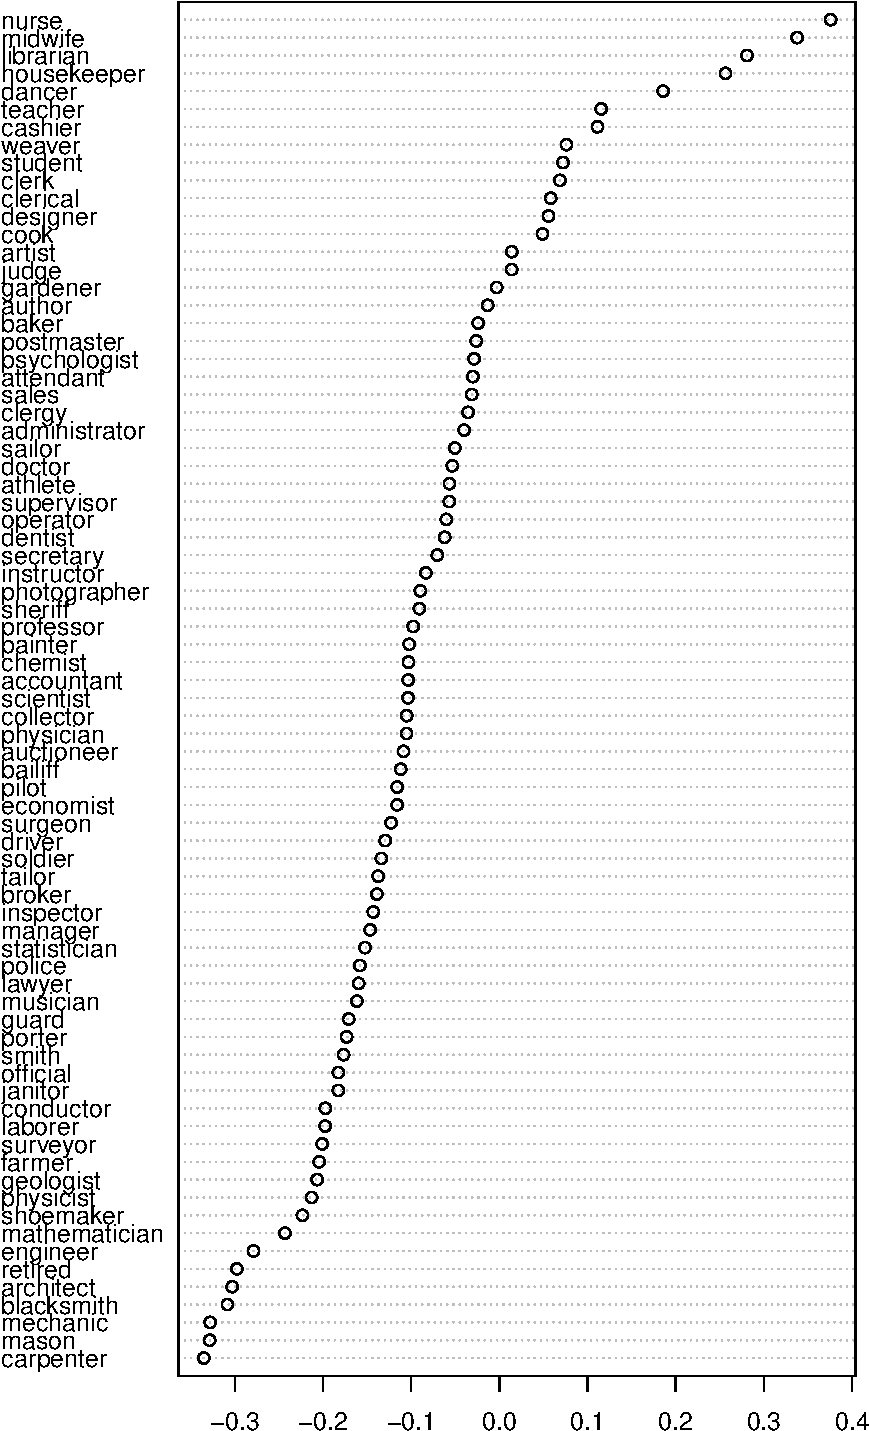
\includegraphics{ica_files/figure-latex/rnd-1.pdf}
\caption{\label{fig:rnd}Bias of words in the target wordset according to relative norm distance}
\end{figure}

The effect size is the sum of all \texttt{P}. As the effect size is negative, it indicates that the concept of occupation is more associated with \(\mathcal{A}\), i.e.~male.

\begin{Shaded}
\begin{Highlighting}[]
\KeywordTok{calculate_es}\NormalTok{(res_rnd_male)}
\end{Highlighting}
\end{Shaded}

\begin{verbatim}
## [1] -6.341598
\end{verbatim}

\hypertarget{relative-negative-sentiment-bias}{%
\subsection{Relative Negative Sentiment Bias}\label{relative-negative-sentiment-bias}}

Relative negative sentiment bias (RNSB) (Sweeney \& Najafian, 2020) takes the same query template as RND. But the technique is not based on a distance metric such as cosine similarity. Instead, the method trained a regularized logistic regression model on the word vectors \(v_{x \in \mathcal{A} \bigcup \mathcal{B}}\) to predict the probability of \(x\) being in \(\mathcal{B}\). The bias is quantified as the relative probability of the word \(s\) for being a word in the wordset \(\mathcal{B}\) (Figure \ref{fig:rnsb}).

\begin{Shaded}
\begin{Highlighting}[]
\NormalTok{res_rnsb_male <-}\StringTok{ }\KeywordTok{query}\NormalTok{(}\DataTypeTok{w =}\NormalTok{ googlenews, }\DataTypeTok{S_words =}\NormalTok{ S, }\DataTypeTok{A_words =}\NormalTok{ A,}
                       \DataTypeTok{B_words =}\NormalTok{ B, }\DataTypeTok{method =} \StringTok{"rnsb"}\NormalTok{)}
\KeywordTok{plot}\NormalTok{(res_rnsb_male)}
\end{Highlighting}
\end{Shaded}

\begin{figure}
\centering
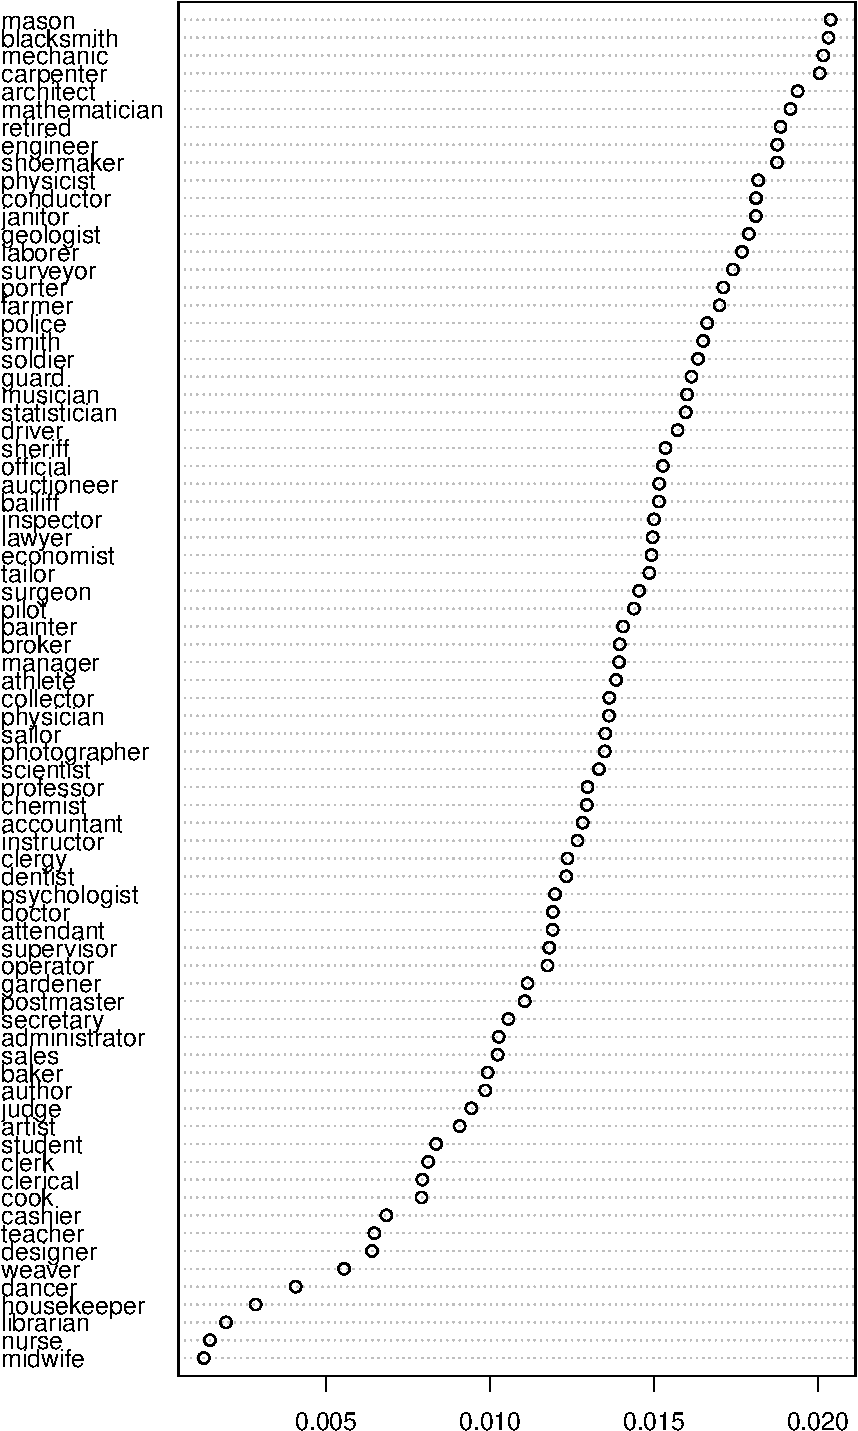
\includegraphics{ica_files/figure-latex/rnsb-1.pdf}
\caption{\label{fig:rnsb}Bias of words in the target wordset according to relative negative sentiment bias}
\end{figure}

The effect size in this case is the Kullback--Leibler divergence of P from the uniform distribution.

\begin{Shaded}
\begin{Highlighting}[]
\KeywordTok{calculate_es}\NormalTok{(res_rnsb_male)}
\end{Highlighting}
\end{Shaded}

\begin{verbatim}
## [1] 0.07398497
\end{verbatim}

\hypertarget{word-embedding-association-test}{%
\subsection{Word Embedding Association Test}\label{word-embedding-association-test}}

Word Embedding Association Test (WEAT) (Caliskan et al., 2017) requires all four wordsets of \(\mathcal{S}\), \(\mathcal{T}\), \(\mathcal{A}\), and \(\mathcal{B}\). The method is modeled after the Implicit Association Test (IAT) (Nosek, Greenwald, \& Banaji, 2005) and it measures the relative strength of \(\mathcal{S}\)'s association with \(\mathcal{A}\) to \(\mathcal{B}\) against the same of \(\mathcal{T}\). The effect sizes calculated from a large corpus, as shown by Caliskan et al. (2017), are comparable to the published IAT effect sizes obtained from volunteers.

In this example, a different \(w\) is used. It is the publicly available GLoVE embeddings made available by the original Stanford Team (Pennington et al., 2014). The same GLoVE embeddings were used in Caliskan et al. (2017). In the following example, the calculation of \enquote{Math. vs Arts} gender bias is reproduced. Please note that for WEAT, the returned object does not contain \texttt{P}. By default, the effect size is standardized so that it can be interpreted the same way as Cohen's D (Cohen, 2013).

\begin{Shaded}
\begin{Highlighting}[]
\KeywordTok{data}\NormalTok{(glove_math) }\CommentTok{# a subset of the original GLoVE word vectors}
\NormalTok{S <-}\StringTok{ }\KeywordTok{c}\NormalTok{(}\StringTok{"math"}\NormalTok{, }\StringTok{"algebra"}\NormalTok{, }\StringTok{"geometry"}\NormalTok{, }\StringTok{"calculus"}\NormalTok{, }\StringTok{"equations"}\NormalTok{, }\StringTok{"computation"}\NormalTok{,}
       \StringTok{"numbers"}\NormalTok{, }\StringTok{"addition"}\NormalTok{)}
\NormalTok{T <-}\StringTok{ }\KeywordTok{c}\NormalTok{(}\StringTok{"poetry"}\NormalTok{, }\StringTok{"art"}\NormalTok{, }\StringTok{"dance"}\NormalTok{, }\StringTok{"literature"}\NormalTok{, }\StringTok{"novel"}\NormalTok{, }\StringTok{"symphony"}\NormalTok{, }\StringTok{"drama"}\NormalTok{,}
       \StringTok{"sculpture"}\NormalTok{)}
\NormalTok{A <-}\StringTok{ }\KeywordTok{c}\NormalTok{(}\StringTok{"male"}\NormalTok{, }\StringTok{"man"}\NormalTok{, }\StringTok{"boy"}\NormalTok{, }\StringTok{"brother"}\NormalTok{, }\StringTok{"he"}\NormalTok{, }\StringTok{"him"}\NormalTok{, }\StringTok{"his"}\NormalTok{, }\StringTok{"son"}\NormalTok{)}
\NormalTok{B <-}\StringTok{ }\KeywordTok{c}\NormalTok{(}\StringTok{"female"}\NormalTok{, }\StringTok{"woman"}\NormalTok{, }\StringTok{"girl"}\NormalTok{, }\StringTok{"sister"}\NormalTok{, }\StringTok{"she"}\NormalTok{, }\StringTok{"her"}\NormalTok{, }\StringTok{"hers"}\NormalTok{, }\StringTok{"daughter"}\NormalTok{)}
\NormalTok{sw <-}\StringTok{ }\KeywordTok{query}\NormalTok{(glove_math, S, T, A, B)}
\NormalTok{sw}
\end{Highlighting}
\end{Shaded}

\begin{verbatim}
## Test type:  weat 
## Effect size:  1.055015
\end{verbatim}

The effect size can also be converted to point-biserial correlation coefficient.

\begin{Shaded}
\begin{Highlighting}[]
\KeywordTok{calculate_es}\NormalTok{(sw, }\DataTypeTok{r =} \OtherTok{TRUE}\NormalTok{)}
\end{Highlighting}
\end{Shaded}

\begin{verbatim}
## [1] 0.4912066
\end{verbatim}

One can also obtain the unstandardized effect size. In the original paper (Caliskan et al., 2017), it is referred to as \enquote{test statistic}.

\begin{Shaded}
\begin{Highlighting}[]
\KeywordTok{calculate_es}\NormalTok{(sw, }\DataTypeTok{standardize =} \OtherTok{FALSE}\NormalTok{)}
\end{Highlighting}
\end{Shaded}

\begin{verbatim}
## [1] 0.02486533
\end{verbatim}

One can also test the statistical significance of the effect size. The original paper suggests an exact test (Caliskan et al., 2017). This exact test is implemented in this package as the function \texttt{weat\_exact}. But the exact test takes a long time to calculate when the number of words in \(\mathcal{S}\) is larger than a few words.

Instead, we recommend the resampling approximation of the exact test. The p-value is extremely close to the reported 0.018.

\begin{Shaded}
\begin{Highlighting}[]
\KeywordTok{weat_resampling}\NormalTok{(sw)}
\end{Highlighting}
\end{Shaded}

\begin{verbatim}
## 
##  Resampling approximation of the exact test in Caliskan et al. (2017)
## 
## data:  sw
## bias = 0.024865, p-value = 0.0154
## alternative hypothesis: true bias is greater than -2.784776e-05
## sample estimates:
##       bias 
## 0.02486533
\end{verbatim}

\hypertarget{conclusion}{%
\section{Conclusion}\label{conclusion}}

This paper demonstrates how \texttt{sweater} can be used to detect biases in word embeddings.

\newpage

\hypertarget{references}{%
\section{References}\label{references}}

\begingroup
\setlength{\parindent}{-0.5in}
\setlength{\leftskip}{0.5in}

\hypertarget{refs}{}
\leavevmode\hypertarget{ref-an2018semaxis}{}%
An, J., Kwak, H., \& Ahn, Y.-Y. (2018). Semaxis: A lightweight framework to characterize domain-specific word semantics beyond sentiment. \emph{arXiv Preprint arXiv:1806.05521}.

\leavevmode\hypertarget{ref-antoniak2021bad}{}%
Antoniak, M., \& Mimno, D. (2021). Bad seeds: Evaluating lexical methods for bias measurement. In \emph{Proceedings of the 59th Annual Meeting of the Association for Computational Linguistics and the 11th International Joint Conference on Natural Language Processing (Volume 1: Long Papers)} (pp. 1889--1904).

\leavevmode\hypertarget{ref-arendt:2013:DDM}{}%
Arendt, F. (2013). Dose-dependent media priming effects of stereotypic newspaper articles on implicit and explicit stereotypes. \emph{Journal of Communication}, \emph{63}(5), 830--851. \url{https://doi.org/10.1111/jcom.12056}

\leavevmode\hypertarget{ref-badilla2020wefe}{}%
Badilla, P., Bravo-Marquez, F., \& Pérez, J. (2020). WEFE: The word embeddings fairness evaluation framework. In \emph{IJCAI} (pp. 430--436).

\leavevmode\hypertarget{ref-boyarskaya2020overcoming}{}%
Boyarskaya, M., Olteanu, A., \& Crawford, K. (2020). Overcoming Failures of Imagination in AI Infused System Development and Deployment. \emph{arXiv Preprint arXiv:2011.13416}.

\leavevmode\hypertarget{ref-brunet2019understanding}{}%
Brunet, M.-E., Alkalay-Houlihan, C., Anderson, A., \& Zemel, R. (2019). Understanding the origins of bias in word embeddings. In \emph{International conference on machine learning} (pp. 803--811).

\leavevmode\hypertarget{ref-caliskan:2017:S}{}%
Caliskan, A., Bryson, J. J., \& Narayanan, A. (2017). Semantics derived automatically from language corpora contain human-like biases. \emph{Science}, \emph{356}(6334), 183--186. \url{https://doi.org/10.1126/science.aal4230}

\leavevmode\hypertarget{ref-cohen2013statistical}{}%
Cohen, J. (2013). \emph{Statistical power analysis for the behavioral sciences}. Academic press.

\leavevmode\hypertarget{ref-dev2019attenuating}{}%
Dev, S., \& Phillips, J. (2019). Attenuating bias in word vectors. In \emph{The 22nd international conference on artificial intelligence and statistics} (pp. 879--887). PMLR.

\leavevmode\hypertarget{ref-du2021assessing}{}%
Du, Y., Fang, Q., \& Nguyen, D. (2021). Assessing the reliability of word embedding gender bias measures. \emph{arXiv Preprint arXiv:2109.04732}.

\leavevmode\hypertarget{ref-eddelbuettel:2013:SRC}{}%
Eddelbuettel, D. (2013). Seamless R and C++ Integration with Rcpp. \url{https://doi.org/10.1007/978-1-4614-6868-4}

\leavevmode\hypertarget{ref-garg:2018:W}{}%
Garg, N., Schiebinger, L., Jurafsky, D., \& Zou, J. (2018). Word embeddings quantify 100 years of gender and ethnic stereotypes. \emph{Proceedings of the National Academy of Sciences}, \emph{115}(16), E3635--E3644. \url{https://doi.org/10.1073/pnas.1720347115}

\leavevmode\hypertarget{ref-knoche2019identifying}{}%
Knoche, M., Popović, R., Lemmerich, F., \& Strohmaier, M. (2019). Identifying biases in politically biased wikis through word embeddings. In \emph{Proceedings of the 30th ACM conference on hypertext and social media} (pp. 253--257).

\leavevmode\hypertarget{ref-kroon2020guilty}{}%
Kroon, A. C., Trilling, D., \& Raats, T. (2020). Guilty by association: Using word embeddings to measure ethnic stereotypes in news coverage. \emph{Journalism \& Mass Communication Quarterly}, 1077699020932304. \url{https://doi.org/10.1177/1077699020932304}

\leavevmode\hypertarget{ref-manzini2019black}{}%
Manzini, T., Lim, Y. C., Tsvetkov, Y., \& Black, A. W. (2019). Black is to criminal as caucasian is to police: Detecting and removing multiclass bias in word embeddings. \emph{arXiv Preprint arXiv:1904.04047}.

\leavevmode\hypertarget{ref-mikolov2013distributed}{}%
Mikolov, T., Sutskever, I., Chen, K., Corrado, G. S., \& Dean, J. (2013). Distributed representations of words and phrases and their compositionality. In \emph{Advances in neural information processing systems} (pp. 3111--3119).

\leavevmode\hypertarget{ref-nosek:2005:UUI}{}%
Nosek, B. A., Greenwald, A. G., \& Banaji, M. R. (2005). Understanding and Using the Implicit Association Test: II. Method Variables and Construct Validity. \emph{Personality and Social Psychology Bulletin}, \emph{31}(2), 166--180. \url{https://doi.org/10.1177/0146167204271418}

\leavevmode\hypertarget{ref-packer2018text}{}%
Packer, B., Mitchell, M., Guajardo-Céspedes, M., \& Halpern, Y. (2018). Text embeddings contain bias. Here's why that matters. Retrieved from \url{https://developers.googleblog.com/2018/04/text-embedding-models-contain-bias.html}

\leavevmode\hypertarget{ref-pennington:2014:G}{}%
Pennington, J., Socher, R., \& Manning, C. (2014). Glove: Global vectors for word representation. \emph{Proceedings of the 2014 Conference on Empirical Methods in Natural Language Processing (EMNLP)}. \url{https://doi.org/10.3115/v1/d14-1162}

\leavevmode\hypertarget{ref-rcore}{}%
R Core Team. (2021). \emph{R: A language and environment for statistical computing}. Vienna, Austria: R Foundation for Statistical Computing. Retrieved from \url{https://www.R-project.org/}

\leavevmode\hypertarget{ref-sales2019media}{}%
Sales, A., Balby, L., \& Veloso, A. (2019). Media bias characterization in brazilian presidential elections. In \emph{Proceedings of the 30th acm conference on hypertext and social media} (pp. 231--240). \url{https://doi.org/10.1145/3345645.3351107}

\leavevmode\hypertarget{ref-rsparse}{}%
Selivanov, D. (2020). \emph{Rsparse: Statistical learning on sparse matrices}. Retrieved from \url{https://CRAN.R-project.org/package=rsparse}

\leavevmode\hypertarget{ref-selivanov2020tex2vec}{}%
Selivanov, D., Bickel, M., \& Wang, Q. (2020). \emph{Text2vec: Modern text mining framework for R}. Retrieved from \url{https://CRAN.R-project.org/package=text2vec}

\leavevmode\hypertarget{ref-sweeney2020reducing}{}%
Sweeney, C., \& Najafian, M. (2020). Reducing sentiment polarity for demographic attributes in word embeddings using adversarial learning. In \emph{Proceedings of the 2020 Conference on Fairness, Accountability, and Transparency} (pp. 359--368).

\leavevmode\hypertarget{ref-wijffelsword2vec}{}%
Wijffels, J. (2021). \emph{Word2vec: Distributed representations of words}. Retrieved from \url{https://CRAN.R-project.org/package=word2vec}

\endgroup


\end{document}
